\section{Pregunta N$^{\circ}$14\qquad Aldo Luna Bueno}

\begin{frame}
	\begin{enumerate}\setcounter{enumi}{13}
		\item

		      Determinar gráficamente el número de raíces reales de la
		      ecuación no lineal
		      \begin{math}
			      \exp\left(x\right)+x=
			      0
		      \end{math}
		      y resuelve usando los métodos de la bisección, la regla
		      falsa y la regla falsa modificada para $\epsilon=10^{-5}$.

	\end{enumerate}

	\begin{solution}

		\begin{figure}
			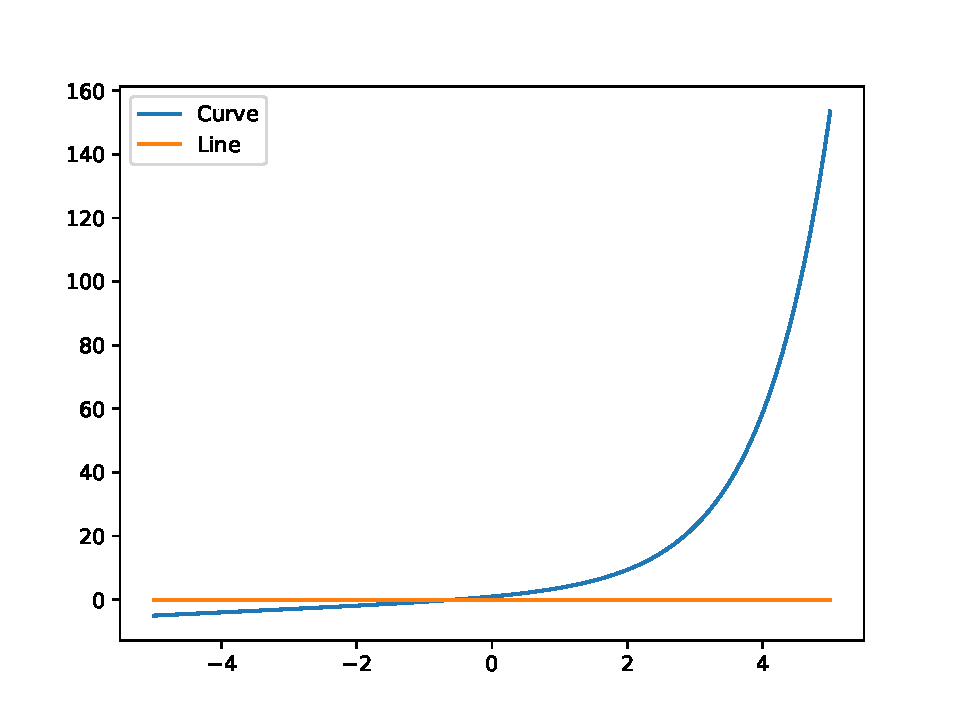
\includegraphics[width=0.5\paperwidth]{p14.pdf}
			% \caption{.}
		\end{figure}
	\end{solution}
\end{frame}

\begin{frame}
	\begin{solution}
		La función
		\begin{math}
			\exp\left(x\right)+x
		\end{math}

		El siguiente teorema nos garantiza la existencia de una raíz en
		un intervalo dadas ciertas condiciones:
		\begin{theorem}
			Si
			\begin{math}
				f\colon
				\left[a,b\right]\subset\mathbb{R}\to
				\mathbb{R}
			\end{math}
			es una función continua y $f\left(a\right)f\left(b\right)<0$,
			entonces existe un $c\in\left]a,b\right[$ tal que
			$f\left(c\right)=0$.
		\end{theorem}

		\begin{figure}
			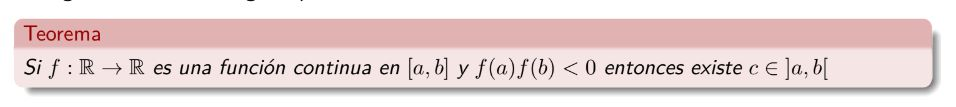
\includegraphics[width=0.5\paperwidth]{p14_teorema_existencia_sol.jpg}
			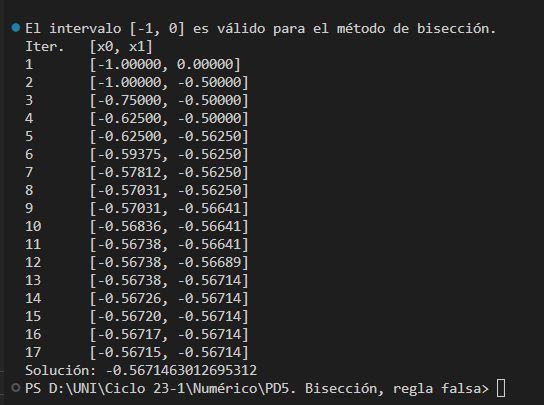
\includegraphics[width=0.5\paperwidth]{p14_bisection_execution.jpg}
		\end{figure}
	\end{solution}
\end{frame}

% \begin{frame}[fragile]
% 	\begin{columns}
% 		\begin{column}{0.48\textwidth}
% 			\inputminted[fontsize=\tiny,firstline=1,lastline=24]{python}{p14_bisection.py}
% 		\end{column}
% 		\begin{column}{0.48\textwidth}
% 			\inputminted[fontsize=\tiny,firstline=26,lastline=52]{python}{p4_sor.py}
% 		\end{column}
% 	\end{columns}
% \end{frame}

\begin{frame}
	\begin{solution}

		\begin{figure}
			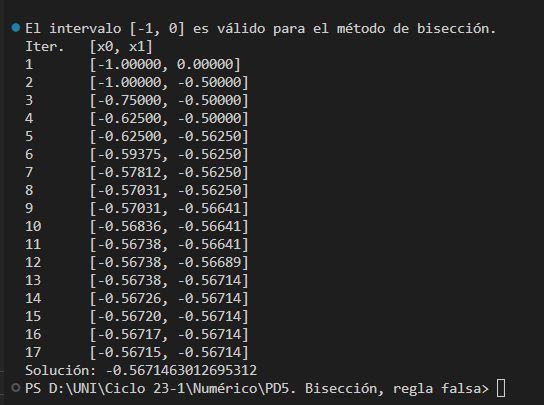
\includegraphics[width=0.5\paperwidth]{p14_bisection_execution.jpg}
			% \caption{.}
		\end{figure}
	\end{solution}
\end{frame}